% Created by tikzDevice version 0.12.3 on 2020-01-31 11:52:48
% !TEX encoding = UTF-8 Unicode
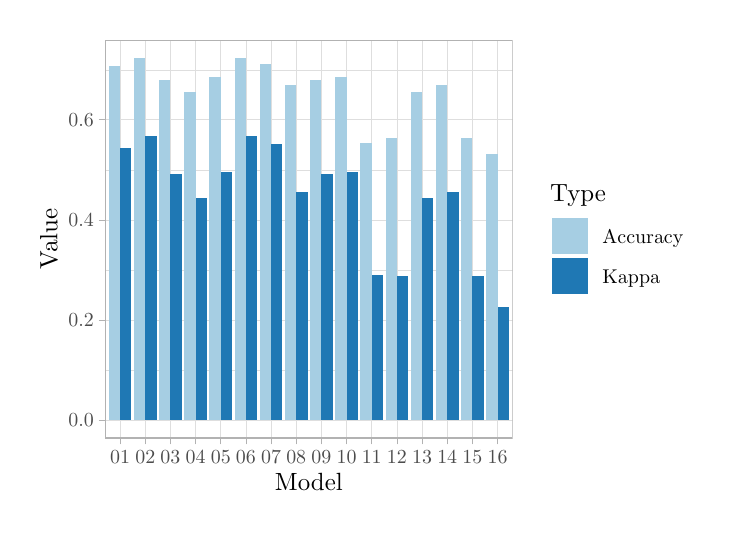
\begin{tikzpicture}[x=1pt,y=1pt]
\definecolor{fillColor}{RGB}{255,255,255}
\path[use as bounding box,fill=fillColor,fill opacity=0.00] (0,0) rectangle (245.72,173.45);
\begin{scope}
\path[clip] (  0.00,  0.00) rectangle (245.72,173.45);
\definecolor{drawColor}{RGB}{255,255,255}
\definecolor{fillColor}{RGB}{255,255,255}

\path[draw=drawColor,line width= 0.5pt,line join=round,line cap=round,fill=fillColor] (  0.00,  0.00) rectangle (245.72,173.45);
\end{scope}
\begin{scope}
\path[clip] ( 27.95, 25.11) rectangle (175.25,168.95);
\definecolor{fillColor}{RGB}{255,255,255}

\path[fill=fillColor] ( 27.95, 25.11) rectangle (175.25,168.95);
\definecolor{drawColor}{gray}{0.87}

\path[draw=drawColor,line width= 0.1pt,line join=round] ( 27.95, 49.73) --
	(175.25, 49.73);

\path[draw=drawColor,line width= 0.1pt,line join=round] ( 27.95, 85.91) --
	(175.25, 85.91);

\path[draw=drawColor,line width= 0.1pt,line join=round] ( 27.95,122.09) --
	(175.25,122.09);

\path[draw=drawColor,line width= 0.1pt,line join=round] ( 27.95,158.27) --
	(175.25,158.27);

\path[draw=drawColor,line width= 0.2pt,line join=round] ( 27.95, 31.64) --
	(175.25, 31.64);

\path[draw=drawColor,line width= 0.2pt,line join=round] ( 27.95, 67.82) --
	(175.25, 67.82);

\path[draw=drawColor,line width= 0.2pt,line join=round] ( 27.95,104.00) --
	(175.25,104.00);

\path[draw=drawColor,line width= 0.2pt,line join=round] ( 27.95,140.18) --
	(175.25,140.18);

\path[draw=drawColor,line width= 0.2pt,line join=round] ( 33.40, 25.11) --
	( 33.40,168.95);

\path[draw=drawColor,line width= 0.2pt,line join=round] ( 42.49, 25.11) --
	( 42.49,168.95);

\path[draw=drawColor,line width= 0.2pt,line join=round] ( 51.59, 25.11) --
	( 51.59,168.95);

\path[draw=drawColor,line width= 0.2pt,line join=round] ( 60.68, 25.11) --
	( 60.68,168.95);

\path[draw=drawColor,line width= 0.2pt,line join=round] ( 69.77, 25.11) --
	( 69.77,168.95);

\path[draw=drawColor,line width= 0.2pt,line join=round] ( 78.87, 25.11) --
	( 78.87,168.95);

\path[draw=drawColor,line width= 0.2pt,line join=round] ( 87.96, 25.11) --
	( 87.96,168.95);

\path[draw=drawColor,line width= 0.2pt,line join=round] ( 97.05, 25.11) --
	( 97.05,168.95);

\path[draw=drawColor,line width= 0.2pt,line join=round] (106.14, 25.11) --
	(106.14,168.95);

\path[draw=drawColor,line width= 0.2pt,line join=round] (115.24, 25.11) --
	(115.24,168.95);

\path[draw=drawColor,line width= 0.2pt,line join=round] (124.33, 25.11) --
	(124.33,168.95);

\path[draw=drawColor,line width= 0.2pt,line join=round] (133.42, 25.11) --
	(133.42,168.95);

\path[draw=drawColor,line width= 0.2pt,line join=round] (142.52, 25.11) --
	(142.52,168.95);

\path[draw=drawColor,line width= 0.2pt,line join=round] (151.61, 25.11) --
	(151.61,168.95);

\path[draw=drawColor,line width= 0.2pt,line join=round] (160.70, 25.11) --
	(160.70,168.95);

\path[draw=drawColor,line width= 0.2pt,line join=round] (169.80, 25.11) --
	(169.80,168.95);
\definecolor{fillColor}{RGB}{31,120,180}

\path[fill=fillColor] ( 33.40, 31.64) rectangle ( 37.49,130.01);
\definecolor{fillColor}{RGB}{166,206,227}

\path[fill=fillColor] ( 29.31, 31.64) rectangle ( 33.40,159.45);
\definecolor{fillColor}{RGB}{31,120,180}

\path[fill=fillColor] ( 42.49, 31.64) rectangle ( 46.59,134.33);
\definecolor{fillColor}{RGB}{166,206,227}

\path[fill=fillColor] ( 38.40, 31.64) rectangle ( 42.49,162.41);
\definecolor{fillColor}{RGB}{31,120,180}

\path[fill=fillColor] ( 51.59, 31.64) rectangle ( 55.68,120.40);
\definecolor{fillColor}{RGB}{166,206,227}

\path[fill=fillColor] ( 47.50, 31.64) rectangle ( 51.59,154.46);
\definecolor{fillColor}{RGB}{31,120,180}

\path[fill=fillColor] ( 60.68, 31.64) rectangle ( 64.77,111.92);
\definecolor{fillColor}{RGB}{166,206,227}

\path[fill=fillColor] ( 56.59, 31.64) rectangle ( 60.68,150.20);
\definecolor{fillColor}{RGB}{31,120,180}

\path[fill=fillColor] ( 69.77, 31.64) rectangle ( 73.87,121.33);
\definecolor{fillColor}{RGB}{166,206,227}

\path[fill=fillColor] ( 65.68, 31.64) rectangle ( 69.77,155.57);
\definecolor{fillColor}{RGB}{31,120,180}

\path[fill=fillColor] ( 78.87, 31.64) rectangle ( 82.96,134.33);
\definecolor{fillColor}{RGB}{166,206,227}

\path[fill=fillColor] ( 74.77, 31.64) rectangle ( 78.87,162.41);
\definecolor{fillColor}{RGB}{31,120,180}

\path[fill=fillColor] ( 87.96, 31.64) rectangle ( 92.05,131.44);
\definecolor{fillColor}{RGB}{166,206,227}

\path[fill=fillColor] ( 83.87, 31.64) rectangle ( 87.96,160.19);
\definecolor{fillColor}{RGB}{31,120,180}

\path[fill=fillColor] ( 97.05, 31.64) rectangle (101.14,114.20);
\definecolor{fillColor}{RGB}{166,206,227}

\path[fill=fillColor] ( 92.96, 31.64) rectangle ( 97.05,152.61);
\definecolor{fillColor}{RGB}{31,120,180}

\path[fill=fillColor] (106.14, 31.64) rectangle (110.24,120.40);
\definecolor{fillColor}{RGB}{166,206,227}

\path[fill=fillColor] (102.05, 31.64) rectangle (106.14,154.46);
\definecolor{fillColor}{RGB}{31,120,180}

\path[fill=fillColor] (115.24, 31.64) rectangle (119.33,121.33);
\definecolor{fillColor}{RGB}{166,206,227}

\path[fill=fillColor] (111.15, 31.64) rectangle (115.24,155.57);
\definecolor{fillColor}{RGB}{31,120,180}

\path[fill=fillColor] (124.33, 31.64) rectangle (128.42, 84.00);
\definecolor{fillColor}{RGB}{166,206,227}

\path[fill=fillColor] (120.24, 31.64) rectangle (124.33,131.71);
\definecolor{fillColor}{RGB}{31,120,180}

\path[fill=fillColor] (133.42, 31.64) rectangle (137.52, 83.80);
\definecolor{fillColor}{RGB}{166,206,227}

\path[fill=fillColor] (129.33, 31.64) rectangle (133.42,133.74);
\definecolor{fillColor}{RGB}{31,120,180}

\path[fill=fillColor] (142.52, 31.64) rectangle (146.61,111.92);
\definecolor{fillColor}{RGB}{166,206,227}

\path[fill=fillColor] (138.42, 31.64) rectangle (142.52,150.20);
\definecolor{fillColor}{RGB}{31,120,180}

\path[fill=fillColor] (151.61, 31.64) rectangle (155.70,114.20);
\definecolor{fillColor}{RGB}{166,206,227}

\path[fill=fillColor] (147.52, 31.64) rectangle (151.61,152.61);
\definecolor{fillColor}{RGB}{31,120,180}

\path[fill=fillColor] (160.70, 31.64) rectangle (164.79, 83.80);
\definecolor{fillColor}{RGB}{166,206,227}

\path[fill=fillColor] (156.61, 31.64) rectangle (160.70,133.74);
\definecolor{fillColor}{RGB}{31,120,180}

\path[fill=fillColor] (169.80, 31.64) rectangle (173.89, 72.35);
\definecolor{fillColor}{RGB}{166,206,227}

\path[fill=fillColor] (165.70, 31.64) rectangle (169.80,127.64);
\definecolor{drawColor}{gray}{0.70}

\path[draw=drawColor,line width= 0.5pt,line join=round,line cap=round] ( 27.95, 25.11) rectangle (175.25,168.95);
\end{scope}
\begin{scope}
\path[clip] (  0.00,  0.00) rectangle (245.72,173.45);
\definecolor{drawColor}{gray}{0.30}

\node[text=drawColor,anchor=base east,inner sep=0pt, outer sep=0pt, scale=  0.72] at ( 23.90, 29.17) {0.0};

\node[text=drawColor,anchor=base east,inner sep=0pt, outer sep=0pt, scale=  0.72] at ( 23.90, 65.34) {0.2};

\node[text=drawColor,anchor=base east,inner sep=0pt, outer sep=0pt, scale=  0.72] at ( 23.90,101.52) {0.4};

\node[text=drawColor,anchor=base east,inner sep=0pt, outer sep=0pt, scale=  0.72] at ( 23.90,137.70) {0.6};
\end{scope}
\begin{scope}
\path[clip] (  0.00,  0.00) rectangle (245.72,173.45);
\definecolor{drawColor}{gray}{0.70}

\path[draw=drawColor,line width= 0.2pt,line join=round] ( 25.70, 31.64) --
	( 27.95, 31.64);

\path[draw=drawColor,line width= 0.2pt,line join=round] ( 25.70, 67.82) --
	( 27.95, 67.82);

\path[draw=drawColor,line width= 0.2pt,line join=round] ( 25.70,104.00) --
	( 27.95,104.00);

\path[draw=drawColor,line width= 0.2pt,line join=round] ( 25.70,140.18) --
	( 27.95,140.18);
\end{scope}
\begin{scope}
\path[clip] (  0.00,  0.00) rectangle (245.72,173.45);
\definecolor{drawColor}{gray}{0.70}

\path[draw=drawColor,line width= 0.2pt,line join=round] ( 33.40, 22.86) --
	( 33.40, 25.11);

\path[draw=drawColor,line width= 0.2pt,line join=round] ( 42.49, 22.86) --
	( 42.49, 25.11);

\path[draw=drawColor,line width= 0.2pt,line join=round] ( 51.59, 22.86) --
	( 51.59, 25.11);

\path[draw=drawColor,line width= 0.2pt,line join=round] ( 60.68, 22.86) --
	( 60.68, 25.11);

\path[draw=drawColor,line width= 0.2pt,line join=round] ( 69.77, 22.86) --
	( 69.77, 25.11);

\path[draw=drawColor,line width= 0.2pt,line join=round] ( 78.87, 22.86) --
	( 78.87, 25.11);

\path[draw=drawColor,line width= 0.2pt,line join=round] ( 87.96, 22.86) --
	( 87.96, 25.11);

\path[draw=drawColor,line width= 0.2pt,line join=round] ( 97.05, 22.86) --
	( 97.05, 25.11);

\path[draw=drawColor,line width= 0.2pt,line join=round] (106.14, 22.86) --
	(106.14, 25.11);

\path[draw=drawColor,line width= 0.2pt,line join=round] (115.24, 22.86) --
	(115.24, 25.11);

\path[draw=drawColor,line width= 0.2pt,line join=round] (124.33, 22.86) --
	(124.33, 25.11);

\path[draw=drawColor,line width= 0.2pt,line join=round] (133.42, 22.86) --
	(133.42, 25.11);

\path[draw=drawColor,line width= 0.2pt,line join=round] (142.52, 22.86) --
	(142.52, 25.11);

\path[draw=drawColor,line width= 0.2pt,line join=round] (151.61, 22.86) --
	(151.61, 25.11);

\path[draw=drawColor,line width= 0.2pt,line join=round] (160.70, 22.86) --
	(160.70, 25.11);

\path[draw=drawColor,line width= 0.2pt,line join=round] (169.80, 22.86) --
	(169.80, 25.11);
\end{scope}
\begin{scope}
\path[clip] (  0.00,  0.00) rectangle (245.72,173.45);
\definecolor{drawColor}{gray}{0.30}

\node[text=drawColor,anchor=base,inner sep=0pt, outer sep=0pt, scale=  0.72] at ( 33.40, 16.10) {01};

\node[text=drawColor,anchor=base,inner sep=0pt, outer sep=0pt, scale=  0.72] at ( 42.49, 16.10) {02};

\node[text=drawColor,anchor=base,inner sep=0pt, outer sep=0pt, scale=  0.72] at ( 51.59, 16.10) {03};

\node[text=drawColor,anchor=base,inner sep=0pt, outer sep=0pt, scale=  0.72] at ( 60.68, 16.10) {04};

\node[text=drawColor,anchor=base,inner sep=0pt, outer sep=0pt, scale=  0.72] at ( 69.77, 16.10) {05};

\node[text=drawColor,anchor=base,inner sep=0pt, outer sep=0pt, scale=  0.72] at ( 78.87, 16.10) {06};

\node[text=drawColor,anchor=base,inner sep=0pt, outer sep=0pt, scale=  0.72] at ( 87.96, 16.10) {07};

\node[text=drawColor,anchor=base,inner sep=0pt, outer sep=0pt, scale=  0.72] at ( 97.05, 16.10) {08};

\node[text=drawColor,anchor=base,inner sep=0pt, outer sep=0pt, scale=  0.72] at (106.14, 16.10) {09};

\node[text=drawColor,anchor=base,inner sep=0pt, outer sep=0pt, scale=  0.72] at (115.24, 16.10) {10};

\node[text=drawColor,anchor=base,inner sep=0pt, outer sep=0pt, scale=  0.72] at (124.33, 16.10) {11};

\node[text=drawColor,anchor=base,inner sep=0pt, outer sep=0pt, scale=  0.72] at (133.42, 16.10) {12};

\node[text=drawColor,anchor=base,inner sep=0pt, outer sep=0pt, scale=  0.72] at (142.52, 16.10) {13};

\node[text=drawColor,anchor=base,inner sep=0pt, outer sep=0pt, scale=  0.72] at (151.61, 16.10) {14};

\node[text=drawColor,anchor=base,inner sep=0pt, outer sep=0pt, scale=  0.72] at (160.70, 16.10) {15};

\node[text=drawColor,anchor=base,inner sep=0pt, outer sep=0pt, scale=  0.72] at (169.80, 16.10) {16};
\end{scope}
\begin{scope}
\path[clip] (  0.00,  0.00) rectangle (245.72,173.45);
\definecolor{drawColor}{RGB}{0,0,0}

\node[text=drawColor,anchor=base,inner sep=0pt, outer sep=0pt, scale=  0.90] at (101.60,  6.25) {Model};
\end{scope}
\begin{scope}
\path[clip] (  0.00,  0.00) rectangle (245.72,173.45);
\definecolor{drawColor}{RGB}{0,0,0}

\node[text=drawColor,rotate= 90.00,anchor=base,inner sep=0pt, outer sep=0pt, scale=  0.90] at ( 10.70, 97.03) {Value};
\end{scope}
\begin{scope}
\path[clip] (  0.00,  0.00) rectangle (245.72,173.45);
\definecolor{fillColor}{RGB}{255,255,255}

\path[fill=fillColor] (184.25, 71.85) rectangle (241.22,122.21);
\end{scope}
\begin{scope}
\path[clip] (  0.00,  0.00) rectangle (245.72,173.45);
\definecolor{drawColor}{RGB}{0,0,0}

\node[text=drawColor,anchor=base west,inner sep=0pt, outer sep=0pt, scale=  0.90] at (188.75,110.63) {Type};
\end{scope}
\begin{scope}
\path[clip] (  0.00,  0.00) rectangle (245.72,173.45);
\definecolor{fillColor}{RGB}{255,255,255}

\path[fill=fillColor] (188.75, 90.80) rectangle (203.21,105.26);
\end{scope}
\begin{scope}
\path[clip] (  0.00,  0.00) rectangle (245.72,173.45);
\definecolor{fillColor}{RGB}{166,206,227}

\path[fill=fillColor] (189.46, 91.51) rectangle (202.49,104.55);
\end{scope}
\begin{scope}
\path[clip] (  0.00,  0.00) rectangle (245.72,173.45);
\definecolor{fillColor}{RGB}{255,255,255}

\path[fill=fillColor] (188.75, 76.35) rectangle (203.21, 90.80);
\end{scope}
\begin{scope}
\path[clip] (  0.00,  0.00) rectangle (245.72,173.45);
\definecolor{fillColor}{RGB}{31,120,180}

\path[fill=fillColor] (189.46, 77.06) rectangle (202.49, 90.09);
\end{scope}
\begin{scope}
\path[clip] (  0.00,  0.00) rectangle (245.72,173.45);
\definecolor{drawColor}{RGB}{0,0,0}

\node[text=drawColor,anchor=base west,inner sep=0pt, outer sep=0pt, scale=  0.72] at (207.71, 95.55) {Accuracy};
\end{scope}
\begin{scope}
\path[clip] (  0.00,  0.00) rectangle (245.72,173.45);
\definecolor{drawColor}{RGB}{0,0,0}

\node[text=drawColor,anchor=base west,inner sep=0pt, outer sep=0pt, scale=  0.72] at (207.71, 81.10) {Kappa};
\end{scope}
\end{tikzpicture}
